\chapter{Classificazione}
In questo capitolo verranno descritti i risultati relativi alle prime due fasi dello studio basate
sulla classificazione: la prima riguardante la classificazione su categorie oggettive, la seconda
su categorie semantiche. Le categorie oggettive riguardano informazioni deducibili dai
metadati dei file audio, come il luogo di registrazione o una fase della giornata. Le categorie
semantiche invece si riferiscono a informazioni ricavate dall’analisi del contenuto dell’audio,
ovvero ai vari suoni identificati presenti nella foresta.

Saranno definiti i gruppi di features utilizzati negli esperimenti, descrivendo poi la tipologia
di classificatore scelto. A seguire, saranno illustrati nel dettaglio i problemi di classificazione
disegnati, ed infine si andrà ad analizzare i risultati ottenuti nei due esperimenti.
L’obiettivo è determinare la parametrizzazione migliore per l’approccio, quali features sono
più efficaci al nostro contesto, e in quali problemi ottengono i risultati migliori. Questo studio
considera gli esperimenti di classificazione precedentemente condotti dai colleghi Ilaria
Ballerini e Andrea Piazza.

Inoltre, viene analizzata la possibilità di aggiungere una fase di filtraggio per alcune
frequenze. L’idea consiste nel rimuovere alcune frequenze preponderanti su ogni audio, che
rappresentano rumore, dovute in maggior parte alle problematiche intrinseche del contesto,
ma anche alla sensibilità dello strumento di misurazione.

\section{Configurazioni \textit{features}}
Nello studio sono state considerate sia le \textit{features} nella loro forma originale, come descritta
nel paragrafo 2.2, sia aggregate. Le \textit{features} originali sono descritte da un numero definito di
componenti (che saranno indicate con \textit{N}). Ogni feature originale è quindi descritta da un
vettore riga di 1x\textit{N} componenti. N dipende dai parametri usati per calcolare lo
spettrogramma.

In particolare sono stati identificati 19 gruppi di \textit{features}:
\begin{itemize}
	\item{11 ORIGINALI (o ORIG), per ognuna delle 11 \textit{features}, utilizzate singolarmente, 1x\textit{N} elementi ciascuna;}
	\item{CONCATENAZIONE ORIGINALI (o CONC.ORIG.), formata dalla concatenazione
	orizzontale delle 11 \textit{features} originali, ottenendo un totale di 11x\textit{N} componenti;}
	\item{CONCATENAZIONE SPETTRALI (o CONC.SPE.), ottenuta dalla concatenazione
	delle componenti delle 5 \textit{features} spettrali, quindi 5x\textit{N} componenti;}
	\item{CONCATENAZIONE TONALI (o CONC.TON.), come la precedente ma
	considerando le 3 \textit{features} della tonalità, ovvero 3x\textit{N} componenti;}
	\item{CONCATENAZIONE TEMPORALI (o CONC.TEM.), come la precedente ma con le
	3 \textit{features} temporali, 3x\textit{N} componenti;}
	\item{CONCATENAZIONE MEDIE ORIGINALI (o CONC.MED.ORIG.), formata dalla
	concatenazione orizzontale delle medie delle 11 \textit{features} originali, quindi 11
	componenti;}
	\item{CONCATENAZIONE MEDIE SPETTRALI (o CONC.MED.SPE.), ottenuta dalla
	concatenazione orizzontale delle medie delle componenti delle 5 \textit{features} spettrali,
	quindi solo 5 componenti;}
	\item{CONCATENAZIONE MEDIE TONALI (o CONC.MED.TON.), come la precedente
	ma utilizzando le 3 \textit{features} tonali, quindi solo 3 componenti;}
	\item{CONCATENAZIONE MEDIE TEMPORALI (o CONC.MED.TEM.), come la
	precedente ma utilizzando le 3 \textit{features} temporali, in totale 3 componenti;}
\end{itemize}

Ai 19 gruppi sopracitati si è tenuto conto anche della relativa versione standardizzata, ovvero
ottenuta dalle componenti processate con la tecnica di standardizzazione \textit{Z Score}, definendo
quindi 38 gruppi: 19 originali e 19 standardizzati. In questo modo, si dispone anche di una
rappresentazione con una scala comune indipendente dalle misurazioni originali.

In aggiunta, i dati sono stati estratti in due forme diverse (ottenendo quindi 78 gruppi di
\textit{features}) basate su diverse finestre temporali scelte per il campionamento nel calcolo dello
spettrogramma: la prima, FS0X, usa una finestra di 32768 campioni, quindi meno di 1
secondo; la seconda, FS1, invece si basa su una finestra di 48000 campioni, corrispondente a
1 secondo.

Nel caso di FS1 sono state estratte 120 componenti (\textit{N}=120): il segnale audio analizzato
presenta una lunghezza temporale di 60 secondi e, per costruire lo spettrogramma lo si
analizza con un intervallo di 1 secondo alla volta, ottenendo 60 finestre. Inoltre, considerando
un passo pari alla metà dell’intervallo, 0.5 secondi, si ottengono altre 60 finestre, per un totale
di 120 campionamenti. Alla stessa modo, è stato fatto per la configurazione FS0X dove,
considerando una finestra più breve, si è ottenuto un maggior numero di componenti
(\textit{N}=176).

La tabella 4.1 riassume i vari gruppi di features considerati.

\begin{table}[htp] 
	\centering
	\begin{tabular}{llrr}
		\toprule
		\textbf{Gruppi}  
		& \textbf{Descrizione}
		& \textbf{\# N x \textit{feature}}
		& \textbf{\# N x \textit{feature}} \\ 
		\textbf{di \textit{features}}
		&  \textbf{\textit{features}} 
		& \textbf{caso FS0X}
		& \textbf{caso FS1} \\
		\midrule
		CONC.ORIG. & Concatenazione originali & 1320 & 1936 \\
		CONC.SPE. & Concatenazione spettrali & 600 & 880 \\
		CON.TON. & Concatenazione tonali & 360 & 528 \\
		CONC.TEM. & Concatenazione temporali & 360 & 528 \\
		CONC.MED.ORIG. & Concatenazione medie originali & 11 & 11 \\
		CONC.MED.SPE. & Concatenazione medie spettrali & 5 & 5 \\
		CONC.MED.TON. & Concatenazione medie tonali & 3 & 3 \\
		CONC.MED.TEM. & Concatenazione medie temporali & 3 & 3 \\
		ORIG & Spectral Centroid & 120 & 176 \\
		ORIG & Spectral Crest Factor & 120 & 176 \\
		ORIG & Spectral Decrease & 120 & 176 \\
		ORIG & Spectral Flatness & 120 & 176 \\
		ORIG & Spectral Flux & 120 & 176 \\
		ORIG & Spectral Roll off & 120 & 176 \\
		ORIG & Spectral Spread & 120 & 176 \\
		ORIG & Spectral Tonal Power Ratio & 120 & 176 \\
		ORIG & Time Zero Crossing Rate & 120 & 176 \\
		ORIG & Time Acf Coeff & 120 & 176 \\
		ORIG & Time Max Acf & 120 & 176 \\
		\bottomrule		
	\end{tabular}	
	\caption{Elenco delle varie \textit{features} utilizzate con relative componenti nelle due configurazioni. Il simbolo \#
		rappresenta la numerosità.}
\end{table}

\section{Dettagli classificatore}
Il classificatore KNN è stato configurato con il valore più semplice, con \textit{k} uguale a 1, facile da
implementare e da comprendere, poiché la decisione della classe si basa unicamente
sull’elemento più vicino (comunemente viene indicata con solo \textit{1-NN}, o solo \textit{NN}). A suo
svantaggio, un valore troppo piccolo, come nel nostro caso, lo rende molto sensibile al
rumore, determinando risultati errati o incongruenze, influenzando l’accuratezza del modello.
Le performance del modello sono state valutate mediante la tecnica di cross validation \textit{Leave
One Out} (LOO). Per semplicità il sistema di classificazione sarà indicato con LOO KNN.

\section{Problemi di classificazione disegnati}
I due problemi di classificazione di questo studio hanno caratteristiche diverse che
illustreremo nei prossimi paragrafi, ma in sostanza si differenziano dalla tipologia di etichette
scelte: la prima cerca di separare classi di natura oggettiva (per esempio il giorno dalla notte),
la seconda invece classi di natura semantica.

\subsection{Problemi con categorie oggettive}
La prima fase propone uno studio sul \textit{dataset} DATA1. Il dataset è privo di annotazione ma
optare per un etichettatura manuale, identificando i vari suoni all’interno, non è considerabile,
sia per l’eccessivo tempo necessario che per la mancanza di risorse. Infatti, come specificato
nell’introduzione, i limiti più ostici consistono da una parte nella difficoltà oggettiva
intrinseca di discriminare elementi all’interno di un \textit{soundscape} e, dall’altra, nella
competenza tecnica necessaria a identificare la biodiversità presente. Per questi motivi, si è
deciso di studiare dei problemi basati su caratteristiche oggettive, cioè su informazioni
deducibili dal contesto dell’oggetto, invece che dal suo contenuto: ad esempio si è tenuto
conto del luogo di registrazione, e della temporalità, come l’ora del giorno, o una fase della
giornata, o del mese.

Sono stati individuati i seguenti problemi:
\begin{itemize}
\item{PR-1.1 YAT. L’obiettivo è individuare il luogo di registrazione, gli \textit{yat}. Si tratta di una
classificazione multiclasse, nel nostro caso 3, relative alle 3 zone in cui sono stati
collocati i microfoni. La cardinalità delle classi vede un 33\% di presenza per ognuno.}
\item{PR-1.2 G/N. Un problema binario che consiste nel discriminare le due fasi
astronomiche principali del giorno, classe G e della notte, classe N. In base alla
latitudine, è stata considerata la fascia oraria del giorno tra le ore 6 e le 17, estremi
compresi. Le ore restanti sono assegnate alla rispettiva classe che identifica la notte.
In tale problema le classi sono equamente bilanciate. }
\item{PR-1.3 AT/R. Un altro problema studiato che considera in un classe i suoni presenti
all’alba e al tramonto, classe AT, e nella seconda le ore rimanenti, classe R. La fascia
oraria considerata per alba è stata identificata tra le ore 5 e le ore 7, estremi compresi,
per il tramonto invece tra le ore 18 e le 20, estremi compresi. L’idea alla base dello
studio di questo problema è che nella prima classe ci possano essere dei suoni
caratterizzanti e simili rispetto al resto della giornata, riconoscibili nell’alba come il
risveglio della natura e nel tramonto come il calare della quiete. Quinn \textit{et alii}
evidenziano l’attività della biofonia in tali fasce della giornata [2]. In questa casistica
la distribuzione si trova in parte sbilanciata sulla classe R, presente per un 70\%.}
\item{PR-1.4 A/T/G/N. Si tratta di una classificazione multiclasse, composta da 4 classi,
discriminando alba, classe A, tramonto, classe T, e le ore rimanenti diurne e notturne,
classi G e N. Le fasce orarie per l’alba e il tramonto sono le medesime presentate
sopra. Le classi A e T sono in una percentuale di distribuzione minore, con circa un
15\% cadauna, rispetto alle classi G e N, che presentano un valore di 40\% e 30\%.}
\item{PR-1.5 M. Problema a 3 classi, che mira a identificare i relativi mesi in cui sono stati
registrati i dati. Per il terzo mese, maggio, è presente un forte squilibrio dovuto alla
mancanza di dati, che si identifica con solo un 4\% dei dati, rispetto a marzo e aprile
con il 49\% e 47\%.}
\item{PR-1.6 MM. Problema binario che mira a discriminare la prima parte del mese (da
inizio mese fino al quindicesimo giorno) dalla seconda (dal sedicesimo giorno fino a
fine mese). La distribuzione è ottimamente bilanciata con circa il 50\% per entrambe le
classi. }
\end{itemize}

In alcune casistiche i dati presentano parti sbilanciate che potrebbero inficiare sulla qualità
del risultato: riguarda maggiormente il problema PR-1.5 M che soffre di una componente poco
rappresentata, il mese di maggio. In questo studio non sono state considerate delle tecniche
conosciute in letteratura per compensare il divario, tuttavia sarebbe sicuramente un aspetto
interessante da esplorare in studi futuri.

\subsection{Problemi con categorie semantiche}
La seconda fase utilizza il \textit{dataset} DATA2, sottoinsieme del \textit{dataset} principale. Come
precedentemente descritto nel capitolo 3, riducendo il set a un numero di dati censibile si è potuto
procedere con una rilevazione manuale dei suoni principali classificando i relativi gruppi. In
questo modo si è potuto disegnare dei problemi di classificazione basati su etichette
semantiche, considerando quindi il contenuto, invece che le informazioni deducibili dai
metadati degli audio (come nella prima fase). 

Sono stati disegnati tre gruppi di problemi di classificazione, suddivisi in base alle classi di
cui sono composti:

\begin{itemize}
	\item{Gruppo PR-2.1. Consiste in una classificazione binaria presenza/assenza, ovvero il
		sistema distingue la presenza o l’assenza di una determinata classe. In questo gruppo
		sono stati formulati quattro problemi, con il relativo rapporto percentuale di
		distribuzione:}
		\begin{itemize}	
			\item{PR-2.1.1 V. Identificazione della classe V del veicolo, in rapporto 42/58;}
			\item{PR-2.1.2 G. Identificazione del suono G dei grilli, con 32/68;}
			\item{PR-2.1.3 P. Identificazione della classe P che caratterizza la pioggia, con un bilanciamento di 37/63;}
			\item{PR-2.1.4 T. Identificazione della classe T che definisce i tuoni, in rapporto 34/66.}
		\end{itemize}
	\item{Gruppo PR-2.2. In questo caso l’obiettivo è discriminare tra due classi distinte. Nel seguente gruppo sono stati disegnati i problemi:}
		\begin{itemize}
			\item{PR-2.2.1 V/P. Vengono messe in corrispondenza ANT/GEO, con le due classi V e P, in rapporto 55/45;}
			\item{PR-2.2.2 V/G. Si confronta ANT/BIO, con le classi V e G, in rapporto 60/40;}
			\item{PR-2.2.3 G/T. Si relaziona BIO/GEO, con le classi G e T, in rapporto 48/52;}
			\item{PR-2.2.4 G/P. Come nel caso precedente, si confronta BIO/GEO, con le classi G e P, in rapporto 46/54;}
		\end{itemize}
	\item{Gruppo PR-2.3. Si tratta di una classificazione a tre classi. Verranno descritti i seguenti problemi che mettono in relazione ANT/BIO/GEO:}
		\begin{itemize}
			\item{PR-2.3.1 V/G/P. Relazionando le classi V, G e P, in un rapporto di 35/30/35;}
			\item{PR-2.3.2 V/G/T. Relazionando le classi V, G e T, in un rapporto di 32/30/38;}
		\end{itemize}
\end{itemize}

Un ultima considerazione, il problema è multi-etichetta, ovvero che ogni audio è
caratterizzato da più suoni, quindi più etichette assegnate allo stesso oggetto. Pertanto, per
proseguire con la stessa metodologia applicata nella prima fase e poter disegnare dei
problemi di classificazione, per i gruppi PR-2 e PR-3, è stato necessario assegnare ad ogni
classe solo gli audio che presentavano quell’unico suono rappresentato dalla classe e non
anche altri suoni del problema: per esempio in una classificazione binaria, in cui vi sono due
classi distinte, non è possibile includere nel problema un audio che contiene entrambi i suoni del problema.
Dunque sono state definite le combinazioni delle classi dove vi era una distribuzione
accettabile delle classi per derivare una casistica interessante da analizzare. Seguendo questa
considerazione, alcune classi sono state escluse da tutti i problemi a causa di una
distribuzione non accettabile:
\begin{itemize}
	\item{le etichette C e U, relative al suono del fiume/cascata e degli uccelli, si trovano in una
	percentuale molto alta, di circa il 94\% e l’81\%;}
	\item{le etichette I e S, relative invece alle interferenze e ai suoni non riconosciuti,
	diversamente, presentano un valore troppo poco rappresentativo, del 3\% e 5\%.}
\end{itemize}

\section{Filtraggio}
I segnali sono stati acquisiti in un contesto reale molto complesso, che comporta la presenza
del rumore. Si è pensato di provare a vedere se poteva migliorare qualcosa filtrando i dati per
ridurre il rumore di fondo rilevato.

In questo paragrafo verrà descritto il filtro applicato alle frequenze dello spettrogramma. È
stato utilizzato un filtraggio classico, che consiste nell’esclusione delle componenti basse o
alte dello spettrogramma. Nel dettaglio, sono stati applicati filtri passa-basso e passa-alto,
che rispettivamente mantengono solo determinate frequenze sotto o sopra un limite definito.
In combinazione si struttura un filtro passa-banda, che mantiene delle frequenze intermedie,
filtrando le superiori e inferiori. Con questi metodi, si dovrebbero eliminare elementi che
potrebbero essere causa di rumore, o che, più semplicemente, risultano irrilevanti per lo
studio. Tale effetto potrebbe determinare un miglioramento della qualità dei dati, e di
conseguenza, una migliore capacità discriminativa del classificatore.

Come metodo di valutazione è stato impiegato lo stesso processo utilizzato per la
classificazione, quindi valutando la percentuale di errore del modello, costruito e testato con i
dati filtrati. È stato utilizzato un singolo problema, testando le varie configurazioni di
features. In particolare lo studio è stato condotto mediante il problema PR-1.1 YAT, ma con
un dataset più ristretto: si è considerato il mese di marzo, con sei audio al giorno ogni quattro
ore, a partire dalle due del mattino, per un totale di 556 file. Si è proceduto in maniera
graduale applicando varie combinazioni di filtri, aumentando progressivamente prima dalla
parte superiore, viceversa poi dalla parte inferiore, proseguendo in convergenza.

L’esito verrà poi esposto nel paragrafo dei risultati, tuttavia si accenna che non è stato
osservato nessun miglioramento.

\section{Risultati}
Prima di esporre e analizzare i risultati ottenuti nei vari problemi di classificazione disegnati,
si discuterà l’esito dell’analisi di filtraggio delle frequenze. Sebbene non abbia portato un
effetto positivo sul segnale, è possibile comunque trarre delle conclusioni interessanti.

\subsection{Filtraggio delle frequenze}
Come descritto precedentemente, sono state testate varie combinazioni di filtri utilizzando
come metodo di valutazione l’errore di classificazione. Per osservare l’andamento complessivo 
dell’applicazione del filtro si è proceduto sintetizzando per ogni test il valore
medio dei risultati ottenuti da tutte le configurazioni di \textit{features}.

Nei grafici delle figure 4.1 e 4.2 è possibile vedere il risultato di questi esperimenti. Sull’asse delle
ascisse si mostra il valore in frequenza utilizzato per filtrare le due zone dello spettrogramma,
nelle varie combinazioni: per esempio, il valore 10 - 20 indica che è stato applicato sulla
parte inferiore un filtro di 10 e sulla parte superiore un filtro di 20. I due grafici mostrano gli
stessi dati ma con un ordinamento diverso: il primo per filtro inferiore ascendente, il secondo
per il superiore. Sull’asse delle ordinate invece è esposta la percentuale di errore medio. Per
potere evidenziare la differenza rispetto alla versione priva di filtraggio, nel grafico si è
aggiunta la voce corrisponde 0-0.

L’osservazione importante è che la differenza tra il caso non filtrato e quelli filtrati è
notevole, e tale contrasto denota un peggioramento significativo del risultato all’aumentare
dei filtri impiegati.

Possiamo tuttavia osservare alcune cose interessanti. La frequenza che ottiene i risultati
migliori, indifferentemente dal filtro, è la FS1.STD: dal secondo grafico è possibile notare la
combinazione di filtri migliore del test derivata dall’utilizzo del solo filtro inferiore nei valori
5, 10 e 15; all’opposto invece la frequenza FS0X.STD ottiene i valori migliori sempre con gli
stessi valori, ma attivi sul filtro superiore (visibile nel grafico  della figura 4.1). La versione FS0X.NOR
(finestra temporale minore di un secondo e dati non normalizzati) ottiene i risultati peggiori,
distaccandosi dei risultati delle versioni FS0X.STD (finestra minore di un secondo e dati
normalizzati) e la FS1.NOR (finestra di un secondo e dati non normalizzati). 

Alla luce di tali risultati, la classificazione è stata poi condotta senza l’utilizzo di filtri.

\begin{center}	
	\begin{figure}[htp]
		\centering
		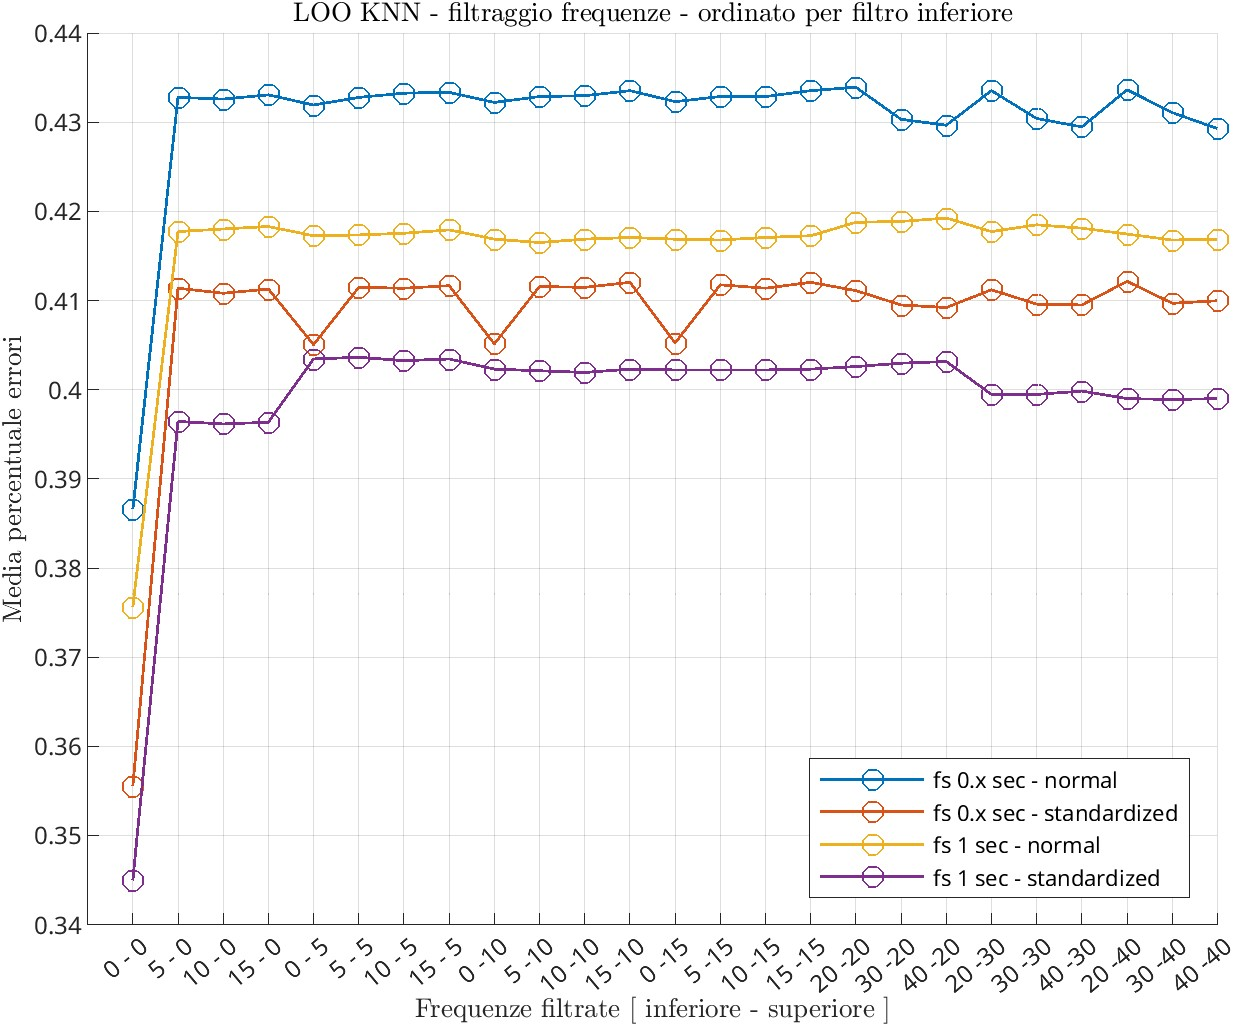
\includegraphics[width=1\textwidth]{img/cap4-filtraggio1.jpg}
		\caption{Risultato filtraggio frequenze ordinato per filtro inferiore. Sull'asse dell'ordinate è esposta la media dell'errore ottenuto per ogni combinazione di filtri presenti sull'asse delle ascisse.}
		\label{fig4.1}
	\end{figure}
\end{center}	
\begin{center}	
	\begin{figure}[htp]
		\centering
		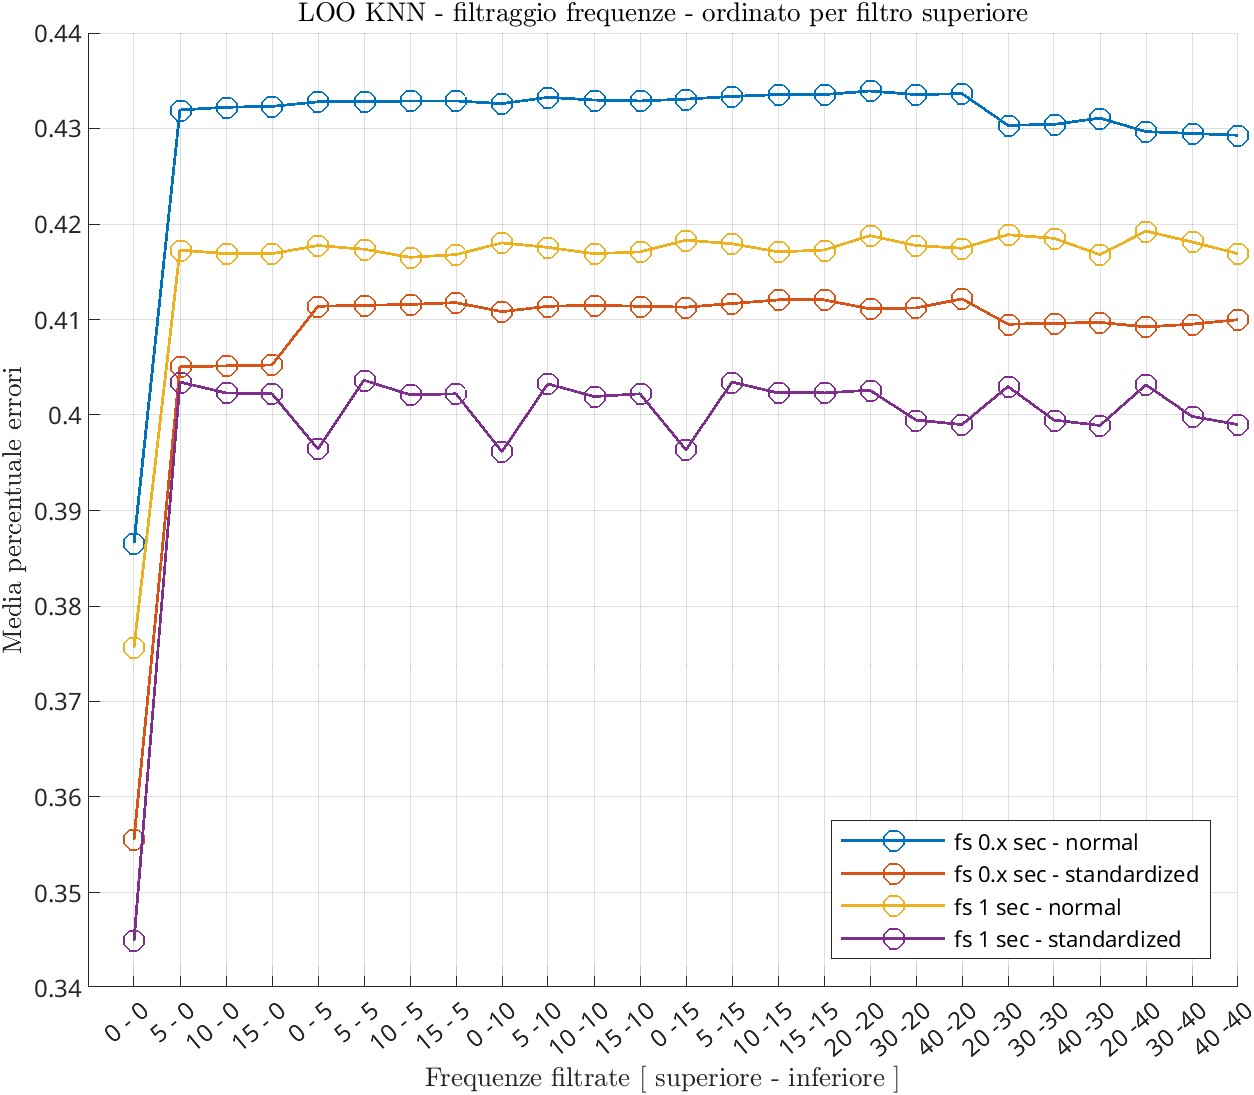
\includegraphics[width=1\textwidth]{img/cap4-filtraggio2.jpg}
		\caption{Risultato filtraggio frequenze ordinato per filtro superiore. Sull'asse dell'ordinate è esposta la media dell'errore ottenuto per ogni combinazione di filtri presenti sull'asse delle ascisse.}
		\label{fig4.2}
	\end{figure}
\end{center}	

\clearpage
\subsection{Risultati problemi con etichette oggettive}
In questa sezione si riportano i risultati della prima analisi di classificazione, basata su
rappresentazione tramite categorie oggettive.

Nel grafico della figura 4.3 si può visualizzare l’esito dei casi sottoposti: sull’asse delle ordinate troviamo
l’errore medio ottenuto dal classificatore, su quello delle ascisse il tipo di problema. Le barre
colorate su ogni problema rappresentano le quattro finestre temporali considerate:
FS0X.NOR, FS1.NOR, FS0X.STD, FS1.STD.

Il miglior risultato lo si individua nel caso PR-1.1 YAT, il problema che che ha come
obiettivo di individuare il luogo di registrazione, gli \textit{yat}. Nella configurazione migliore si
ottiene un errore del 0.9\%. Questo problema è l’unico tra quelli con categorie oggettive che
tratta della discriminazione del luogo. Sicuramente ha goduto, oltre alle peculiarità della zona
in sé, persino delle caratteristiche dello stato dello strumento di misurazione. Si può
ipotizzare che elementi come le interferenze o le condizioni meteorologiche, colpendo
indifferentemente i vari sensori, abbiano marchiato il prodotto segnando maggiormente uno
tra questi rispetto agli altri per un determinato periodo temporale: hanno caratterizzato una
parte del registrato e contribuito ad accrescere le già notabili differenze, definite
dall’ambiente circostante, con il resto dei dispositivi. Non di meno, un altro dettaglio
importante riguarda il suono rappresentante dell’elemento cascata C, che è quasi
onnipresente, poiché lo si ritrova nella totalità delle registrazioni, ma in versioni eterogenee
tra i dispositivi, dato che sono posizionati a distanze differenti dalla sorgente del rumore. E’
possibile affermare che una discriminazione basata sul luogo ha sicuramente beneficiato di
queste condizioni rispetto alle altre casistiche.

D’altra parte, anche le tipologie sviluppate sulla temporalità hanno ottenuto complessivamente 
dei buoni risultati. L’idea alla base dei casi PR-1.2 G/N e PR-1.3 AT/R di
caratterizzare i periodi astronomici dell’alba e del tramonto, ha portato delle conclusioni
interessanti, in particolare nel secondo, che si basava proprio sul discriminare questi due
momenti principali rispetto al resto della giornata. Nelle migliori configurazioni si è ottenuto
un errore del 14\% per PR-1.2 G/N e del 25\% per PR-1.3 AT/R. Pur sapendo che in un
contesto naturale presentano delle caratteristiche sonore uniche, si rende noto, che,
diversamente dalle aspettative, il sistema di classificazione non è stato così efficace per il
problema PR-1.4 A/T/G/N, risultato con la maggiore percentuale di errori in una media del
50\%. Ovviamente c’è il numero delle classi (4) superiore rispetto agli altri scenari, portando
una notevole complessità quindi una minore capacità di generalizzazione. Inoltre, è possibile
ipotizzare che il risultato sia stato determinato anche dalla riduzione della quantità dei dati di
addestramento da cui estrarre un modello identificativo di ogni classe: avendo un numero
finito di campioni all’aumentare della classi diminuisce il numero di oggetti per descriverle.
Per quanto riguarda le finestre considerate, si evidenzia dal grafico, mediante i colori delle
barre, come la FS1.STD (finestra minore di un secondo normalizzata) abbia ottenuto le
migliori prestazioni in ogni problema di classificazione. Si può ipotizzare che la finestra più
ampia permetta di cogliere maggiori dettagli di interesse nel contesto: una finestra con
maggiore risoluzione potrebbe risultare vantaggiosa per lo studio. A tale risoluzione anche il
rumore potrebbe risultare meno influente, non facendo quindi risaltare determinati elementi
irrilevanti per la classificazione. Allo stesso modo, anche l’altra versione standardizzata
FS0X.STD ha riportato un esito accettabile e abbastanza simile alla finestra appena descritta.
Se consideriamo l’effetto della standardizzazione, possiamo osservare come entrambe le
versioni standardizzate hanno conseguito un errore minore rispetto alle controparti regolari.
Si considera però che, la finestra più corta, ma con dati standardizzati, FS0X.STD, nella
maggioranza dei casi ha ottenuto dei risultati migliori della finestra più ampia ma con dati
normali, FS1S.NOR. Quindi si può dedurre che per il contesto la scelta corretta sia una
combinazione tra la finestra più ampia e dati standardizzati.

Il grafico in figura 4.4 mostra la medesima situazione sotto un'altra prospettiva cioè dal punto di vista
delle \textit{features}, sintetizzando per ogni configurazione il suo errore medio tra i vari problemi
disegnati. Nei gruppi con le features singole ORIG gli errori per tipologia di finestra si
discostano di poco, diversamente che nelle forme combinate dove le versioni standardizzate
sono maggiormente incisive. Lo si può notare nel gruppo CONC.MED.ORIG., che ottiene i
migliori risultati in entrambe le versioni standardizzate con un errore medio intorno al 18\%.
Riassume le caratteristiche essenziali dei tre gruppi SPE/TON/TEM, servendosi di un numero
ristretto di \textit{features}, undici in questo caso. Un insieme di componenti ridotto, riduce la
complessità del modello, rendendolo più robusto, aumentando la sua interpretabilità e
ottenendo una migliore generalizzazione.

\begin{center}	
	\begin{figure}[htp]
		\centering
		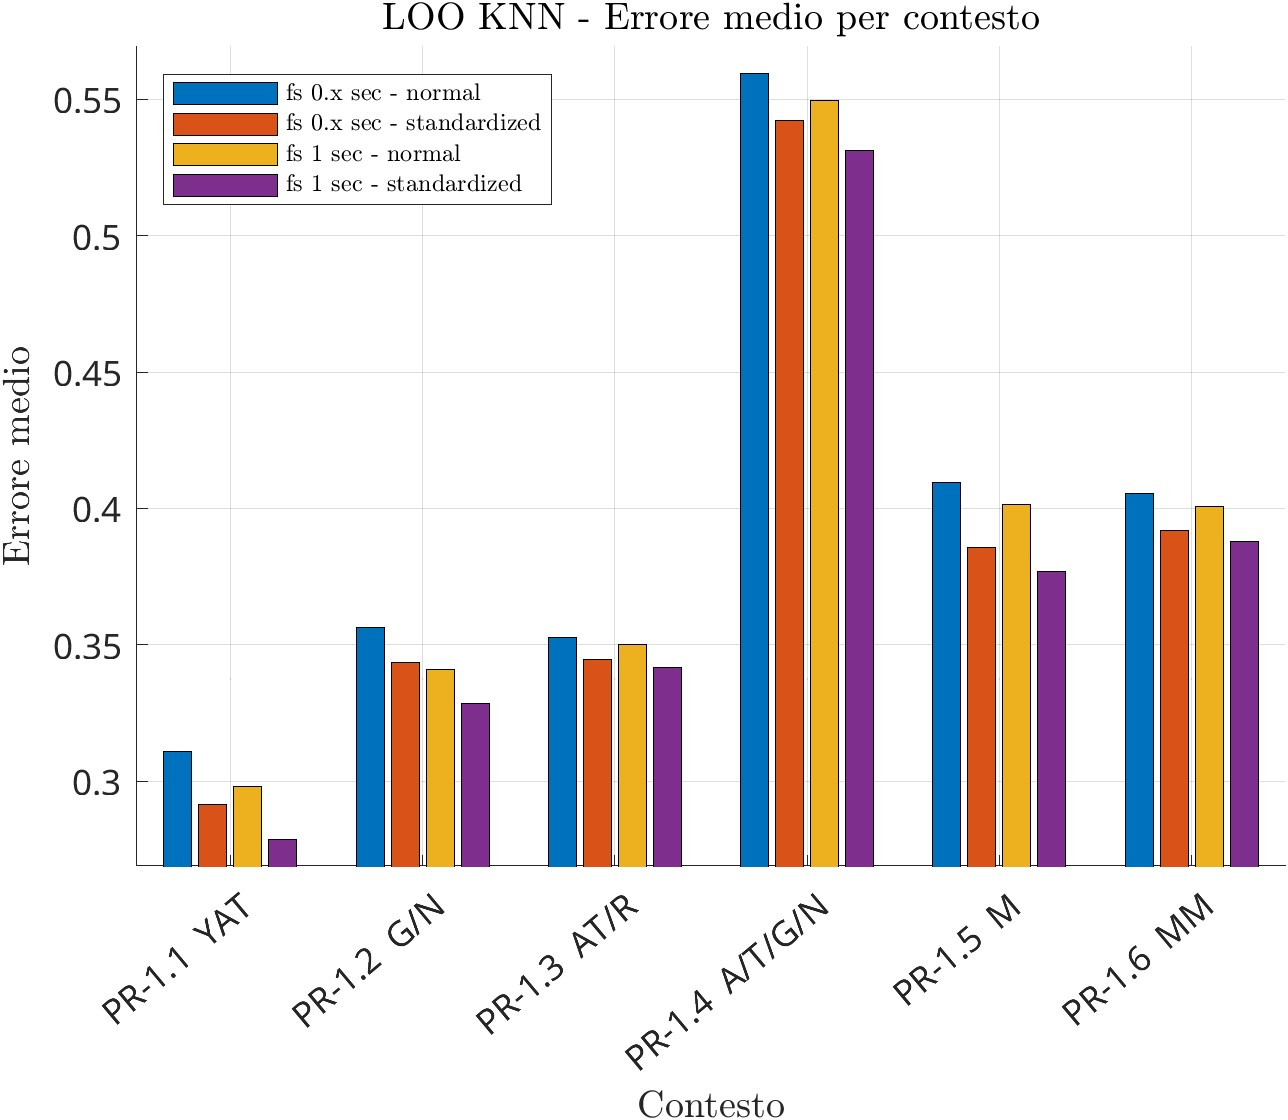
\includegraphics[width=1\textwidth]{img/cap4-classificazione_fase1_binaria.jpg}
		\caption{Errore medio nei problemi di classificazione disegnati per le quattro finestre temporali considerate.}
		\label{fig4.3}
	\end{figure}
\end{center}	
\begin{center}	
	\begin{figure}[htp]
		\centering
		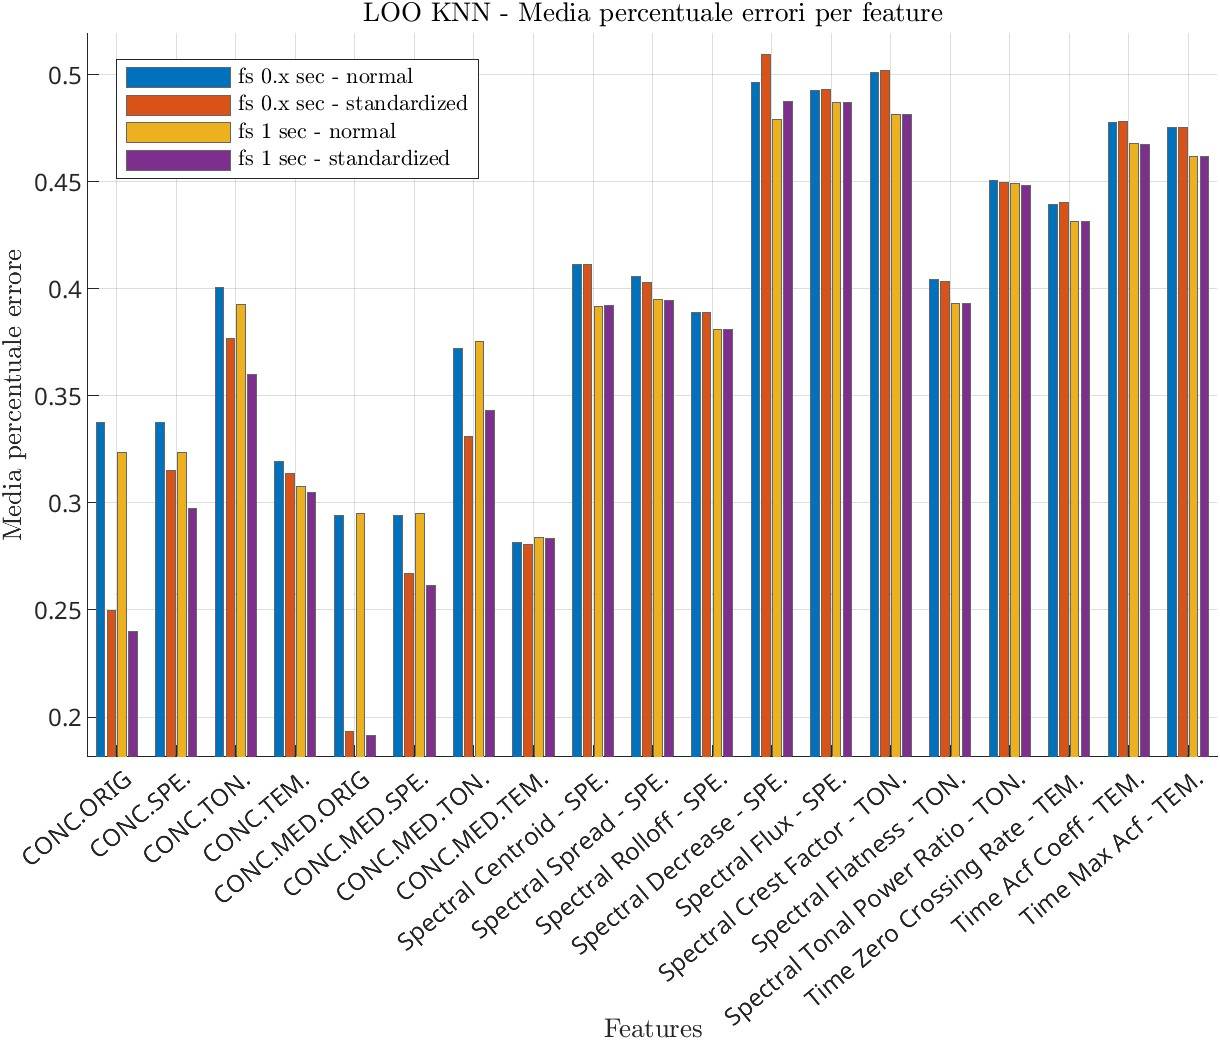
\includegraphics[width=1\textwidth]{img/cap4-classificazione_fase1_features.jpg}
		\caption{Errore medio dei problemi di classificazione dal punto di vista delle features per le quattro finestre.}
		\label{fig4.4}
	\end{figure}
\end{center}

\cleardoublepage
\subsection{Risultati problemi con etichette semantiche}
Nel corrente paragrafo andremo ad analizzare i risultati della seconda fase di classificazione
che analizza i problemi rappresentati da categorie semantiche. Come precedentemente
affermato, tali casistiche sono state disegnate in una condizione multi-etichetta, ovvero che
ogni audio è caratterizzato da più suoni, quindi più etichette assegnate allo stesso oggetto.

In generale possiamo sostenere che gli esperimenti con la versione standardizzata ottengono
una media di errore minore rispetto alla controparte non normalizzata, nel dettaglio, la
versione FS1.STD primeggia costantemente. Lo si può osservare nel grafico in figura 4.5 che riassume
gli esiti dei problemi disegnati, sintetizzando per ogni configurazione il suo errore medio tra i
vari problemi disegnati. È chiaro che il valore medio in queste analisi permette di trarre una
visione generale dell’insieme. Tuttavia, si sottolinea che a causa dello scarso risultato di
alcune \textit{features}, l’esito può essere sbilanciato. Per questo verranno comunque evidenziati i
dati che spiccano rispetto al gruppo, ma che potrebbero discostarsi in alcuni casi dai quelli
esposti nel grafico. Si evidenzia che, siccome nel grafico i casi di classificazione a tre classi
hanno avuto un errore fuori scala rispetto alla media generale, si è deciso per comprimere una
parte dell’asse delle ordinate per ottenere una migliore visione dell’insieme: la zona
compressa riguarda i valori tra 0.44 e 0.54 evidenziata sul grafico mediante una barra
orizzontale grigia, la fascia intermedia presente tra i risultati a due e tre classi.
A seguire saranno descritti nel dettaglio i tre gruppi elencati nel paragrafo 4.4.2.

In merito ai casi di classificazione PR-2.1 (binari) che discriminano la presenza/assenza di
una determinata classe, i risultati mostrano un errore medio nei problemi disegnati intorno al
39\% di errore. È possibile notare che la classe V ottiene un lieve miglioramento con la
finestra FS0X.NOR, diversamente dagli altri casi, dove invece vediamo sempre prevalere la
versione FS1.STD.

In questo gruppo i problemi con i migliori risultati riguardano i suoni appartenenti alla GEO,
delle classi T e P nei problemi PR-2.1.3 P con il 24\% di errore e PR-2.1.4 T con il 26\%. Si
evidenzia il risultato delle feature CONC.MED.SPE, che primeggia in entrambe le frequenze,
con una media di errori pari al 33\%, e in un posizione molto vicina anche la feature
CONC.MED.ORIG. Il loro risultato lo si può notare nel grafico in figura 4.6, che mette in evidenza il
comportamento delle features trasversalmente ai casi sottoposti, con una media sui valori. È
possibile notare che anche CONC.SPE. e CONC.ORIG, hanno ottenuto in generale un buon
risultato. In questo gruppo la BIO sembra essere stata caratterizzata dalle \textit{features} spettrali.

Per quanto concerne il gruppo PR-2.2, classificazione binaria ma con due classi distinte i
risultati sono soddisfacenti per il nostro contesto con una media di errore del 39\%.
Probabilmente anche perché le classi sono più bilanciate. Questi problemi hanno permesso di
valutare gli insiemi ANT/BIO/GEO in contrapposizione a coppie, evidenziando delle
differenze rilevanti. È possibile notare l’ANT in contrasto con la GEO, nel problema
PR-2.2.1 V/P con una media di errore del 43\%, dove si ottengono risultati peggiori rispetto al
confronto con la BIO, nel problema PR-2.2.2 V/G con una media di errore del 38\%: è
ipotizzabile supporre che il suono dei grilli, essendo discontinuo come il suono del veicolo,
ha permesso al sistema di poterli discriminare più facilmente, a differenza invece, del suono
della pioggia, che si mantiene persistente. Allo stesso modo, lo ritroviamo nella correlazione
di BIO con ANT, in PR-2.2.1 V/P con una media di errore del 43\%, e BIO con GEO, in
PR-2.2.4 G/P con una media di errore del 37\%: si nota nel primo una maggiore difficoltà,
come appena evidenziato. La minima presenza del suono di veicoli all’interno del dato ha
sicuramente influito sul modello, quindi è possibile ipotizzare che il suono dei grilli con la
pioggia abbia permesso un confronto simile al suono del veicolo con la pioggia, essendo
entrambi molto percepibili. Differentemente, potendo valutare due casi relativi allo stesso
confronto BIO/GEO, in PR-2.2.3 G/T e PR-2.2.4 G/P, è osservabile un comportamento
simile, con valori leggermente migliori dei casi sopra esposti, con un media di errore del 37\%
e nelle configurazioni migliori un errore del 20\%. Si ipotizza che l’origine simile, per T e P,
pur essendo suoni diversi, converga in un intervallo di frequenze simili, che rispecchiano la
GEO. Da un punto di vista delle features, si evidenzia che, in maniera simile al primo gruppo
i risultati migliori sono dati dalla versione standardizzata per CONC.ORIG e CONC.SPE per
quanto riguarda il problema PR-2.2.4 G/P, con un 20\% medio di errore. Invece con un 25\%
negli altri casi per le stesse versioni ma con le medie concatenate in CONC.MED.ORIG e
CONC.MED.SPE.. Tali valori si possono notare nel grafico in figura 4.6, che espone i risultati dalla
prospettiva delle \textit{features}.

Nei casi di classificazione a tre classi, PR-2.3.1 V/G/P e PR-2.3.2 V/G/T, i risultati si sono
rivelati inferiori alle aspettative con un errore medio di circa del 54\%. Le classi pur essendo
bilanciate, si trovavano in quantità significativamente minori. Inoltre, il numero di classi, pari
a tre, ha complicato ulteriormente il modello, unitamente ai possibili disturbi causati dagli
altri suoni non inerenti al problema. Dal punto di vista delle features invece si nota un
comportamento diverso dai casi precedenti. Infatti, nel primo caso PR-2.3.1 V/G/P otteniamo
i migliori risultati con le \textit{feature} CONC.MED.ORIG, nella versione standardizzata in
particolare, invece nel secondo caso PR-2.3.2 V/G/T, vediamo protagonista la CONC.MED.TON 
con un errore del 40\% circa, per entrambe le finestre ed entrambe le forme
normali e standardizzate. Il grafico in figura 4.8 ci propone i dati del gruppo dal punto di vista delle
\textit{features}.

È possibile presupporre che ogni risultato sia stato influenzato negativamente dalla presenza
di altri suoni non considerati nel problema in esame, come, allo stesso tempo, la quantità
limitata di dati a disposizione per classe potrebbe conseguire un scarso addestramento
condizionando la capacità di generalizzazione del discriminatore.

In sintesi, possiamo evidenziare che i tutti i casi analizzati le feature CONC.MED.ORIG si
dimostrano tra le migliori per descrivere i vari casi esposti, seguite da CONC.MED.SPE. nel
particolare dei casi binari, e da CONC.MED.TON. per i casi ternari. In particolare,
esprimono al meglio il loro potenziale nella versione con la finestra FS1.STD, che è risultata
superiore nella maggioranza delle casistiche.

\vspace{12pt}

\begin{center}	
	\begin{figure}[htp]
		\centering
		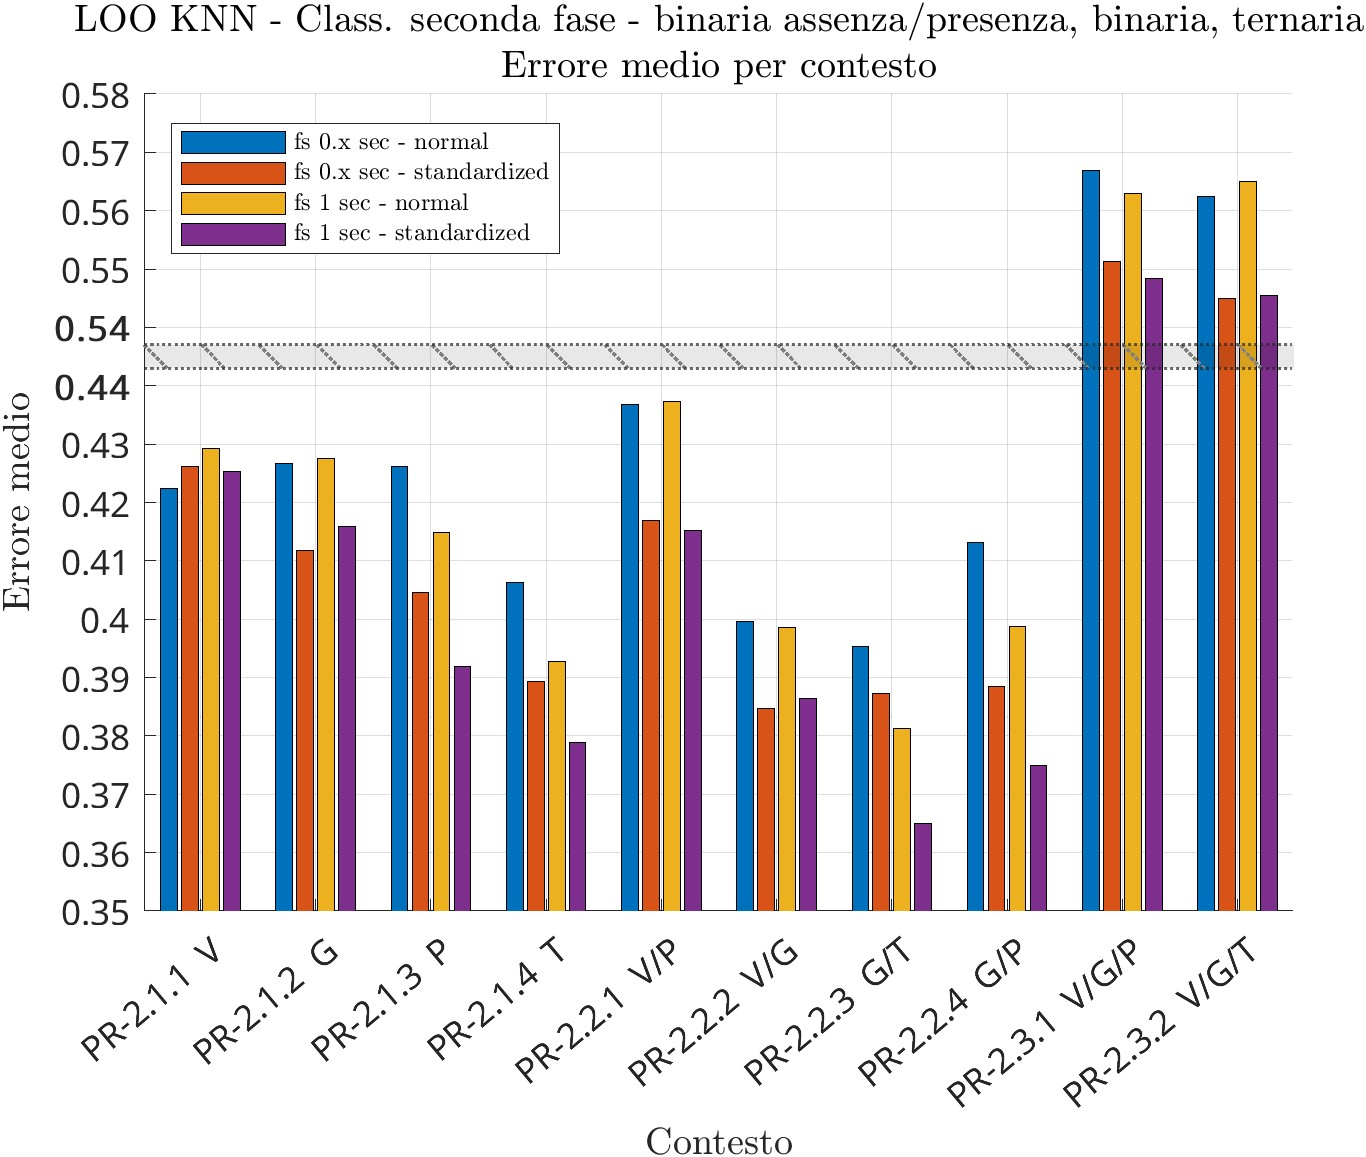
\includegraphics[width=0.9\textwidth]{img/cap4-classificazione_fase2_problemi.jpg}
		\caption{Risultati problemi di classificazione con categorie semantiche. Le barre colorate identificano per
			ogni problema le quattro finestre impiegate. Il risultato esposto è la sintesi dell’errore medio ottenuto con tutte
			le configurazioni di features. La barra grigia orizzontale indica una zona in cui i dati sono stati compressi per
			ottenere una migliore visione del grafico.}
		\label{fig4.5}
	\end{figure}
\end{center}	
\begin{center}	
	\begin{figure}[htp]
		\centering
		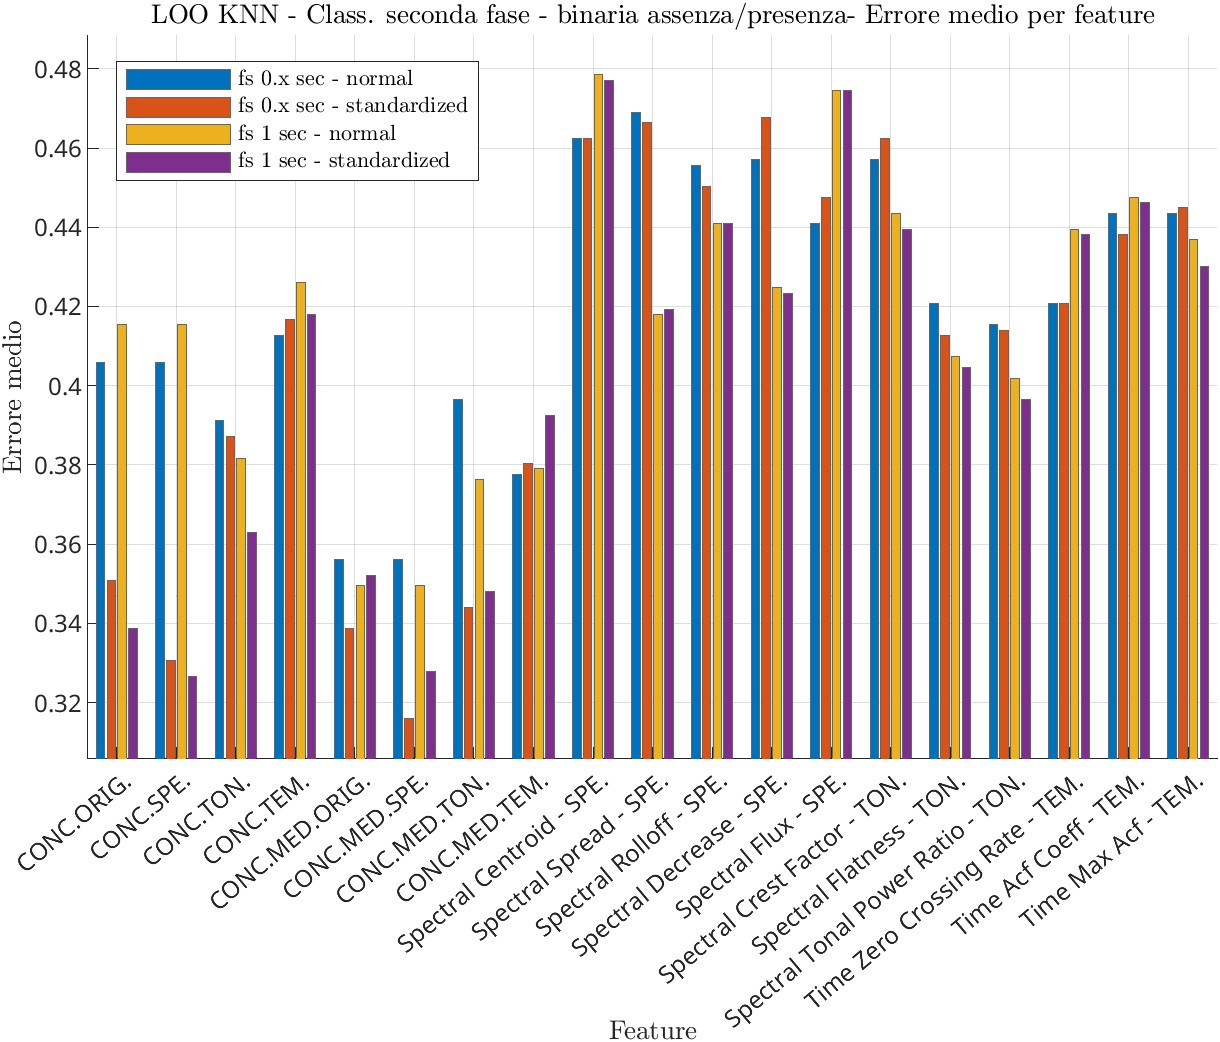
\includegraphics[width=1\textwidth]{img/cap4-classificazione_fase2_features_binaria_presenza.jpg}
		\caption{Risultati problemi di classificazione binaria presenza/assenza con categorie semantiche dal punto
			di vista delle \textit{features}. Le barre colorate identificano per ogni \textit{features} le quattro finestre impiegate. Il risultato
			esposto è la sintesi dell’errore medio tra i vari problemi disegnati.}
		\label{fig4.6}
	\end{figure}
\end{center}
\begin{center}	
	\begin{figure}[htp]
		\centering
		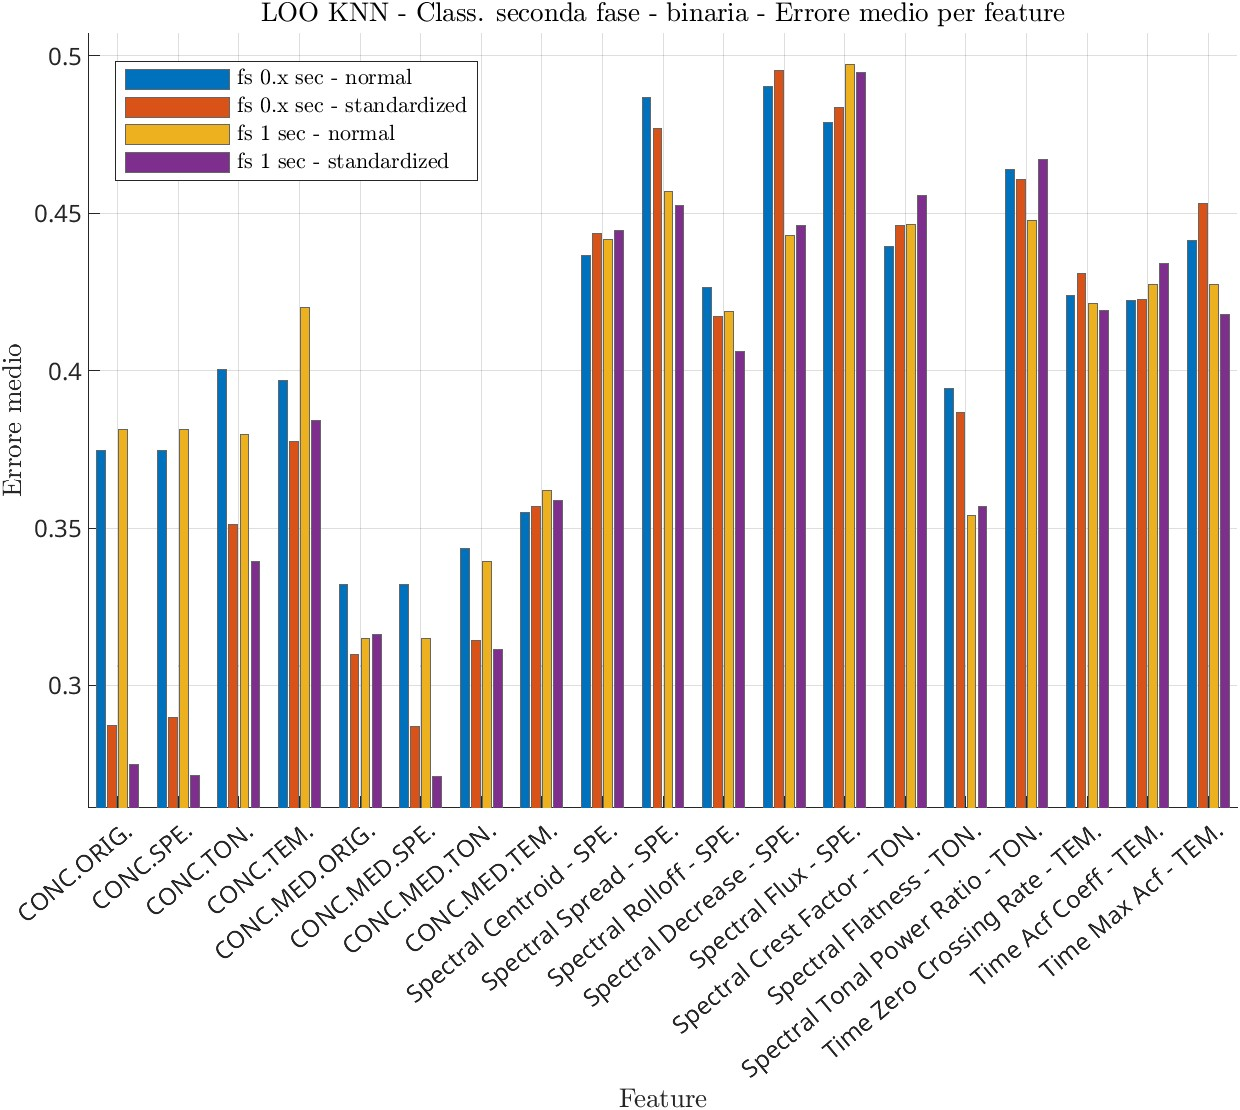
\includegraphics[width=1\textwidth]{img/cap4-classificazione_fase2_features_binaria_distinte.jpg}
		\caption{Risultati problemi di classificazione binaria a due classi distinte con categorie semantiche dal punto di
			vista delle \textit{features}. Le barre colorate identificano per ogni \textit{features} le quattro finestre impiegate. Il risultato
			esposto è la sintesi dell’errore medio tra i vari problemi disegnati.}
		\label{fig4.7}
	\end{figure}
\end{center}	
\begin{center}	
	\begin{figure}[htp]
		\centering
		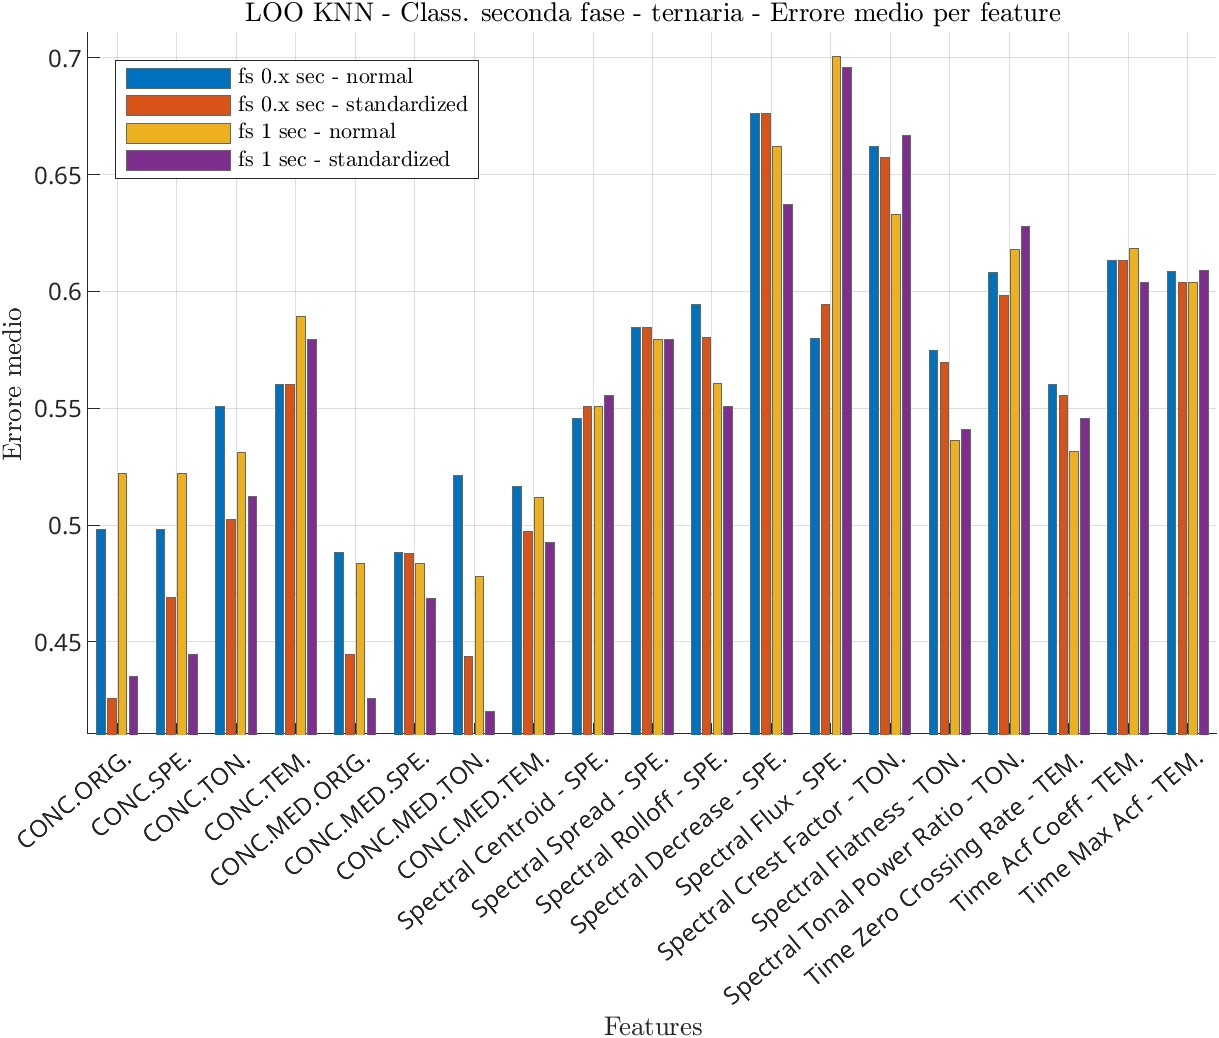
\includegraphics[width=1\textwidth]{img/cap4-classificazione_fase2_features_ternaria.jpg}
		\caption{Risultati problemi di classificazione a tre classi con categorie semantiche dal punto di
			vista delle \textit{features}. Le barre colorate identificano per ogni \textit{features} le quattro finestre impiegate. Il risultato esposto è la sintesi dell’errore medio tra i vari problemi disegnati.}
		\label{fig4.8}
	\end{figure}
\end{center}
